\documentclass[tikz]{standalone}
\usepackage[complete,amssymbols,amsbb,eufrak,nofontinfo,
             subscriptcorrection,zswash,mtpscr]{mtpro2}
\usepackage{textgreek}
\renewcommand{\pi}{\text{\textpi}}
\usetikzlibrary{shadings,3d,positioning,patterns,mindmap,fadings}
\usepackage{ctex,amsmath,fontspec}
\definecolor{tou}{RGB}{94,125,89}
\definecolor{author}{RGB}{225,244,225}
\definecolor{title}{RGB}{255,253,127}
\definecolor{left}{RGB}{148,176,107}
\definecolor{body}{RGB}{144,192,108}
\definecolor{body1}{RGB}{90,182,90}
\definecolor{topbot}{RGB}{60,92,76}
\newcommand{\yp}[1]{{\CJKfontspec{印品赤壁赋体}#1}}
\newcommand{\fz}[1]{{\CJKfontspec{方正黑体简体}#1}}
\setmainfont{Times New Roman}
\everymath{\displaystyle}
\newcommand{\ii}{\,\!\mathrm i\,\!}
\usepackage[hidelinks]{hyperref}
\begin{document}
\begin{tikzpicture}
\node[minimum width=17.7cm,minimum height=25cm,inner sep=0pt,outer sep=0pt,](box){};
\fill[body,top color=body1,bottom color=body](box.north west)--(box.north east)--(box.south east)--(box.south west)--cycle;
\draw[help lines,step=0.8cm,opacity=0.4](-8.85,-12.5)grid(8.85,12.5);
\node[align=center,text=author] at (box.center)
{\zihao{-2}\fz{向禹} \tikz{\draw(0.25,0.25)circle(0.25);\draw(0.25,0.25)circle(0.2);} \fz{译}
};
\fill[tou](-8.85,6.5)[bend left=25]to(8.85,10.8)--(box.north east)--(box.north west)--cycle;
\fill[left color=left,right color=tou](-8.85,6.5)[bend left=24]to(8.85,10.6)
--(8.85,9.6)[bend right=23]to(-8.85,6.5);
\node[text=title,align=center,scale=3]at(0,4){\fz{1994-2018年国际大学生}\\[-0.2cm]\fz{数学竞赛}};
\node[text=orange!20,align=center,scale=1.5]at(0,2){\fz{International Mathematics Competition}\\[-0.2cm]\fz{for University Students (1994-2018)}};
\node[opacity=0.5,draw,rounded corners] at(-2,7.8){$\int_a^bf(x)\,\mathrm dx=F(b)-F(a)$};
\node[opacity=0.5] at(5.4,7.8){\tikz{\draw[-stealth](-0.3,0)--(0,0)node[below left]{$O$}--(3.6,0)node[below=2pt]{$x$};
\draw[-stealth](0,-0.42)--(0,2)node[left]{$y$};
\draw(0,1.3)node[left]{$A$}..controls(1.4,0.6)and(2.2,2.4)..(2.8,1.7)node[right]{$B$}
--(2.8,0)node[below]{$C$};\node at(0.65,1.4){$f(x)$};}};
\node[opacity=0.6] at(-3.5,-3.5)
{
\scalebox{0.5}{\begin{tikzpicture}
  \path [
    mindmap,
    text = white,
    level 1 concept/.append style =
      {font=\Large\bfseries, sibling angle=90},
    level 2 concept/.append style =
      {font=\normalsize\bfseries},
    level 3 concept/.append style =
      {font=\small\bfseries},
    tex/.style     = {concept, ball color=white,
      font=\Huge\bfseries},
    分析/.style = {concept, ball color=purple!90!black},
    formats/.style = {concept, ball color=blue!50!black},
    systems/.style = {concept, ball color=red!90!black},
    editors/.style = {concept, ball color=orange!90!black}
  ]
  node [tex,text=blue!80] {\scalebox{1.4}{IMC}} [clockwise from=0]
    child[concept color=green!50!black, nodes={分析}] {
      node {分析} [clockwise from=90]
        child { node {数学分析} }
        child { node {实分析} }
        child { node {复分析} }
        child { node {泛函分析} }
        }
    child [concept color=red, nodes={systems}] {
      node {图论组合}}
    child [concept color=blue, nodes={formats}] {
      node {代数} [clockwise from=240]
        child { node {线性代数} }
        child { node {抽象代数} }
         child { node {初等数论} }}
    child [concept color=orange, nodes={editors}] {
      node {概率论} };
\end{tikzpicture}}
};
\node[opacity=0.4]at(5.5,-2){
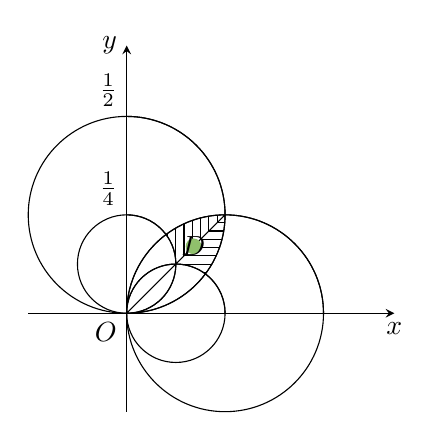
\begin{tikzpicture}[scale=10]
\begin{scope}
\clip (0,0) arc (-90:0:1/8) arc (90:180:1/8);
\fill[pattern=horizontal lines]
(0,0) arc (-90:0:1/8) --(1/16,1/16) arc (90:0:1/16);
\fill[pattern=vertical lines]
(0,0) arc (180:90:1/8) --(1/16,1/16) arc (0:90:1/16);
\end{scope}\node[below left](0,0){$O$};
\draw [-stealth](-1/8,0)--(0.34,0);\draw [-stealth](0,-1/8)--(0,0.34);
\node[below]at(0.34,0){$x$};\node[left]at(0,0.34){$y$};
\draw (0,0) arc (-90:90:1/8) (0,0) arc (-90:90:1/16)
(0,0) arc (180:0:1/8) (0,0) arc (180:0:1/16) (0,0)--(1/8,1/8);
\fill[fill=body](0.085,0.085)node[inner sep=0pt]{$D$}circle(0.01);
\draw(0,1/8)circle(1/8);\draw(0,1/16)circle(1/16);
\draw(1/8,0)circle(1/8);\draw(1/16,0)circle(1/16);
\node[above left]at(0,1/4){$\tfrac12$};\node[above left]at(0,1/8){$\tfrac14$};
\end{tikzpicture}
};
\node[opacity=0.3] at(3,-6.5){$\left( \sum_{n=1}^{\infty}{a_{n}^{2}} \right) \left( \sum_{n=1}^{\infty}{b_{n}^{2}} \right) \geqslant \left( \sum_{n=1}^{\infty}{a_nb_n} \right) ^2$};
\node[opacity=0.3] at(0,-8){$f(z)=\frac1{2\pi\ii}\oint_C\frac{f(\xi)}{\xi-z}\,\mathrm d\xi$};
\fill[tou](-8.85,-10.5)--(-8.85,-12.5)--(8.85,-12.5)--(8.85,-10.5)--cycle;
\node[anchor=north,align=left,text=author]at(0,-10.7){

\begin{tikzpicture}[color=author]
\draw[very thick,rounded corners](0,0)--(0,1.3)--(1.3,1.3)--(1.3,0)--cycle;
\fill(0.65,1.08)circle(0.12);
\fill(0.15,0.93)--(0.65,0.8)--(1.15,0.93)--(1.15,0.98)--(0.65,0.85)--(0.15,0.98)--cycle;
\foreach \x in{-0.12cm,-0.16cm,-0.2cm}
\fill[yshift=\x](0.15,0.93)--(0.65,0.8)--(1.15,0.93)--(1.15,0.98)--(0.65,0.85)
--(0.15,0.98)--cycle;
\foreach \x in{-0.32cm,-0.36cm,-0.4cm,-0.44cm,-0.48cm,-0.52cm,-0.56cm,-0.6cm,-0.64cm}
\fill[yshift=\x](0.15,0.93)--(0.65,0.8)--(1.15,0.93)--(1.15,0.98)--(0.65,0.85)
--(0.15,0.98)--cycle;
\end{tikzpicture}
\parbox{4cm}{\vspace{-1.2cm}
\scalebox{1.7}{\yp{无名出版社}}\\[-2mm]
\scalebox{0.5}[1]{PUBLISHING HOUSE OF NONAME}\\[-2mm]
\href{yuxtech.github.io}{yuxtech.github.io}
}};
\end{tikzpicture}

\end{document} 